% bar-476.tex
% See the folder on flat-faced cylinders

\section{Pressure on a flat-faced cylinder}
\label{bar-476-sec}
%
This example models the bar gauge type of pressure sensor 
as used in the expansion-tube facilities.
It also shows the application of a multiple-block grid to
describe the flow domain (Figure\,\ref{bar-geometry-fig}) around a flat-faced
cylinder whose axis is aligned with the free-stream flow direction.
The free-stream Mach number is 4.76 to match one of the higher Mach number
conditions reported in Ref.\cite{kendall_1959a}.

\begin{figure}[htbp]
\begin{center}
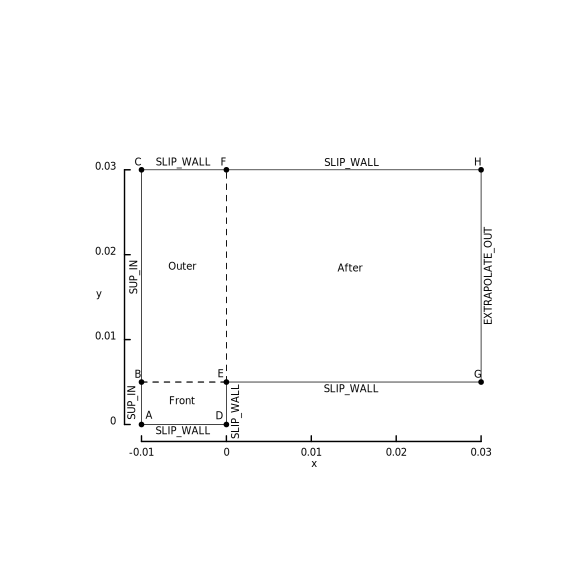
\includegraphics[width=12cm,viewport=75 78 397 328,clip=true]{../2D/bar-476/bar-layout.pdf}
\end{center}
\caption{Schematic diagram of the full flow domain around the flat-faced cylinder.}
\label{bar-geometry-fig}
\end{figure}

The simulation is started with low pressure stationary gas throughout
the domain and the inflow conditions are applied to the west boundaries
of blocks ``Front'' and ``Outer''.
After allowing 50\,$\mu$s for the flow to reach steady state, 
the pressure distribution throughout the domain is shown in
Fig.\,\ref{bar-pressure-mach-fig}.
The stand-off distance was determined by searching
for the pressure jump along the row of cells adjacent to the centreline.
See the \texttt{locate\_shock.awk} script below.
If the trigger for the pressure jump is 200\,kPa, the stand-off distance is 2.815\,mm but, 
if we use a level of 1.5\,MPa, the estimated stand-off distance is 2.756\,mm.
The difference is about 70\% of one cell width. 

\begin{figure}[htbp]
\mbox{
\includegraphics[width=0.5\textwidth]{../2D/bar-476/bar-p-field.png}
\includegraphics[width=0.5\textwidth]{../2D/bar-476/bar-Mach-field.png}
}
\caption{Pressure and Mach number within the flow domain at 50\,$\mu$s.}
\label{bar-pressure-mach-fig}
\end{figure}

Figure~\ref{bar-pressure-profile-fig} shows the distribution of pressure
across the face of the cylinder.  
The simulation data agrees closely with Kendall's measurements 
except in the region the sharp corner where there is inadequate resolution
and an absence of viscous effects in the simulation.

\begin{figure}[htbp]
\begin{center}
\includegraphics[width=10cm,viewport=68 53 400 291,clip=true]{../2D/bar-476/bar_norm_p.pdf}
\end{center}
\caption{Normalised pressure across the face of the cylinder
         compared with experimental measurements\,\cite{kendall_1959a}.}
\label{bar-pressure-profile-fig}
\end{figure}

\newpage
\subsection{Input script (.py)}
\topbar
\lstinputlisting[language={}]{../2D/bar-476/bar.py}
\bottombar

\newpage
\subsection{Shell scripts}
\label{bar-sh-files}
\topbar
\lstinputlisting[language={}]{../2D/bar-476/prepare_simulation.sh}
\bottombar

\noindent
\topbar
\lstinputlisting[language={}]{../2D/bar-476/run_simulation.sh}
\bottombar

\noindent
\topbar
\lstinputlisting[language={}]{../2D/bar-476/post_simulation.sh}
\bottombar

\newpage
\subsection{Awk scripts}
\label{bar-awk-files}
\topbar
\lstinputlisting[language={}]{../2D/bar-476/normalize.awk}
\bottombar

\noindent
\topbar
\lstinputlisting[language={}]{../2D/bar-476/locate_shock.awk}
\bottombar


\subsection{Notes}
\begin{itemize}
\item The \texttt{mbcns2} version of this simulation 
      reaches a final time of 50\,$\mu$s in 2932 steps and,
      on a Pentium-M 1.73\,Ghz system, this takes 19\,min, 27\,s of CPU time.
      This is equivalent to 17.8\,$\mu$s per cell per predictor-corrector
      time step.
\item The \texttt{Eilmer3} simulation takes 2929 steps and 19\,min, 6\,s on 
      an Intel Core 2 Duo E8400 at 3GHz.
      We have some optimization to do...
\end{itemize}
